% !TeX root = bachelorarbeit.tex
\begin{Bemerkung}
	Die beiden folgenden Abschnitte bauen im Wesentlichen auf den beiden Vorlesungen 'Einführung in das Wissenschaftliche Rechnen' (SS 2019) und 'Finite Elemente Methoden' (WS 2019/2020) von Herrn Prof. Dr. Wieners auf. Dem entsprechend sind als Quellen neben \cite{brenner2007mathematical} und 
	\cite{braess2013finite} vor allem die Mitschriebe zu den oben genannten Vorlesungen, sowie die Berichte zum Rechnerpraktikum mit M++ \cite{siteM++} zu nennen.
\end{Bemerkung}
Wie bereits in obigem Abschnitt erwähnt, sollen sich die nächsten beiden Abschnitte damit beschäftigen, wie wir die oben beschriebenen Probleme für ein festes $\omega \in \Omega$ numerisch lösen können. 
Ein Überblick über alle möglichen Verfahren, welche zur Lösung der beiden Probleme geeignet sind, würde den Rahmen dieser Thesis sprengen. Wir wollen deshalb im Folgenden auf eine Möglichkeit eingehen diese Berechnung numerisch durchzuführen. Insbesondere werden dabei jene Verfahren beschrieben, welche wir auch später innerhalb der MLMC Methode in M++ nutzen wollen.
Da wir in diesen beiden Abschnitte $\omega \in \Omega$ ohnehin fest halten, genügt es zudem das deterministische Problem zu betrachten. \newline
Sowohl das hybride Finite Elemente Verfahren, welches wir zur Lösung des Potentialströmungsproblem nutzen wollen, als auch das Discontinuous Galerkin Vefahren, mit dessen Hilfe wir das Transportproblem lösen wollen, bauen auf der Finite Elemente Theorie auf. 
Diese ist im Wesentlichen in der zweiten Hälfte des 20. Jahrhunderts entstanden, ist aber bis heute in praktischer wie auch in theoretischer Sicht aktuell.
Die Grundidee ist hierbei die vorliegenden Rand-Anfangswertaufgaben in einem passenden endlichen Unterraum zu lösen. Dabei löst man sich auf analytischer Seite zunächst oft von einzelnen Regularitäts- und Differenzierbarkeitsbedingungen und führt einen sogenannten schwachen Lösungsbegriff ein (vergleiche Abschnitt 2.1). Statt nun aber solch eine schwache Lösung in einem unendlich dimensionalen Funktionenraum, wie beispielsweise in den Sobolevräumen $W^{1,2}(\mathbb{D})$ oder $W_0^{1,2}(\mathbb{D})$ zu bestimmen, zieht man sich auf endliche Unterräume zurück. \newline
Die folgende Definition entstammt \cite{brenner2007mathematical} und geht ursprünglich (1978) auf Ciarlet zurück.
\begin{Definition}\
	Sei
	\begin{itemize}
		\item $K \subseteq \R^d$ eine beschränkte abgeschlossene Menge mit einem nichtleeren Inneren und stückweise stetig differenzierbarem Rand 
		\item $\mathcal{P}$ ein endlich dimensionaler Funktionenraum auf K
		\item $\mathcal{N} = \{N_1,N_2,\dots,N_k \}$ eine Basis für $\mathcal{P}^{'}$
	\end{itemize}
	Dann heißt $(K,\mathcal{P},\mathcal{N})$ ein finites Element.
\end{Definition}

Wir wollen im Folgenden diese theoretische Definition zwar im Hinterkopf behalten, aber wie in \cite{braess2013finite} meist nur mit den sogenannten Finite-Elemente-Räumen arbeiten. 
Dabei wird eine geeignete Zerlegung $\mathfrak{K} = \{K_1,K_2,\dots, K_M \}$ von $\mathbb{D}$ in endlich viele Teilgebiete gewählt. 
Anschließend betrachten wir einen endlichen Raum von Funktionen, die eingeschränkt auf diese Teilgebiete von einfacher Gestalt sind, beispielsweise bieten sich oft polynomielle Darstellungen niedrigen Grades an. 
Ein solches Teilgebiet $K \in \mathfrak{K}$ nennen wir Finites Element oder auch Zelle und fordern implizit verbunden mit dem betrachteten Funktionenraum die Erfüllung der obigen Definition. \newline
Im Falle $\mathbb{D} \subseteq \R^2$ kommen so z.B. Dreiecke oder Vierecke in Frage, in $\mathbb{D} \subseteq \R^3$ können Tetraeder, Würfel, Quader und andere genutzt werden. \newline
Sei nun $\mathbb{D} \subseteq \R ^2$ zudem ein polygonales Gebiet, um eine einfache Zerlegung in Dreiecke oder Vierecke zu gewährleisten.

\begin{Definition}
	\begin{enumerate}
		\item Eine Zerlegung $\mathfrak{K} = \{ K_1,K_2,\dots,K_M\}$ von $\mathbb{D}$ in Dreiecks- oder Viereckselemente heißt zulässig, wenn folgende Eigenschaften erfüllt sind:
		\begin{itemize}
			\item $\overline{\mathbb{D}} = \bigcup_{i=1}^M K_i$
			\item Für $i \neq j$ ist $K_i\cap K_j$
			\begin{enumerate}
				\item ein gemeinsamer Eckpunkt von $K_i$ und $K_j$
				\item eine gemeinsame Kante von $K_i$ als auch von $K_j$
				\item oder $K_i\cap K_j= \emptyset$
			\end{enumerate}
			
		\end{itemize}
		\item Wir schreiben oft $\mathfrak{K}_h$ anstatt $\mathfrak{K}$, wenn jedes Element einen Durchmesser von höchstens $2h$ besitzt [Vorlesung h = max diam K was passt besser]
	\end{enumerate}
\end{Definition}

\begin{figure}[h]
	\centering
	\captionabove{Zulässige Triangulierung und unzulässige Triangulierung mit hängendem Knoten}
	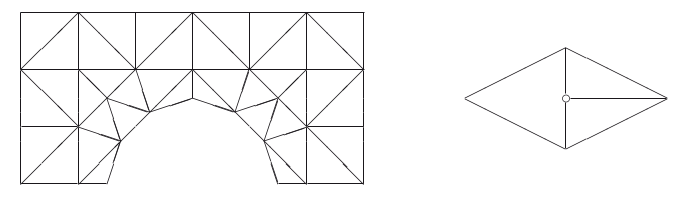
\includegraphics[width=0.8\textwidth]{triangulierung.png} \\
	Abbildung aus \cite{braess2013finite} Seite 58
\end{figure}

\subsubsection{Schwache Formulierung}
Betrachten wir also die deterministische Version des Potentialströmungsproblem:
\[ \text{Bestimme } u:\overline{\mathbb{D}} \to \R \text{ und } q: \overline{\mathbb{D}} \to \R^2 \text{ mit } \newline \]
\[\setlength\arraycolsep{1pt}
\text{(PS)}\begin{cases} 
\begin{array}{rlcr}
\dive q     &= 0                 &\text{ ,} \text{in } \mathbb{D} &(1)\\
q           &= - \kappa \nabla u &\text{ ,} \text{in }\mathbb{D} &(2)\\
u           &= u_D               &\text{ ,} \text{auf } \Gamma_D \\
-q \cdot n  &= g_N               &\text{ ,} \text{auf } \Gamma_N 
\end{array}
\end{cases} 
\]
In Satz (ref todo) haben wir gesehen, dass wir in obiger Formulierung Gleichung (1) mit Testfunktionen $\Phi \in W_0^{1,2}(\mathbb{D})$ und Gleichung (2) mit Testfunktionen $\Psi \in ??? $ multiplizieren und anschließend über $\mathbb{D}$ integrieren können und so eine äquivalente schwache Formulierung herleiten:
\begin{align*}
	\int_{\mathbb{D}} \dive(q) \Phi \dx &= 0 \text{ für alle Testfunktionen } \Phi : \mathbb{D} \to \R \\
	\int_{\mathbb{D}} (q + \kappa \nabla u) \cdot \Psi \dx &= 0 \text{ für alle Testfunktionen } \Psi : \mathbb{D} \to \R^2
\end{align*}
Da $\kappa$ weiter symmetrisch positiv definit ist, lässt sich letztere Gleichung zu 
\begin{align*}
	&\int_{\mathbb{D}} \kappa^{-1} (q + \kappa \nabla u) \cdot \Psi \dx = 0 \text{ für alle Testfunktionen } \Psi : \mathbb{D} \to \R^2\\
	\Leftrightarrow \qquad &\int_{\mathbb{D}} \nabla u \cdot \Psi \dx = - \int_{\mathbb{D}} (\kappa^{-1}q)\cdot \Psi \dx \text{ für alle Testfunktionen } \Psi : \mathbb{D} \to \R^2
\end{align*}
umformen. Außerdem wollen wir nun noch die Dirichlet-Randbedingungen $u = u_D \text{ auf } \Gamma_{\text{D}}$ einfließen lassen. Dazu verwenden wir den Satz von Gauß:

=========
TODO
=========
\[ \int_{\partial\Omega} (u\Psi) \cdot n \da \stackrel{\text{Gauß}}{=} 
 \int_{\Omega} \dive(u\Psi) \dx = \int_{\Omega} \nabla u \cdot \Psi \dx + \int_{\Omega} u \dive(\Psi) \dx \quad (\Psi:\Omega \to \R^2) \]
Wählen wir nun unseren Ansatzraum so, dass  für die Funktion $ \Psi: \Omega \to \R$ gilt $ \Psi \cdot n = 0 \text{ auf } \Gamma_N $. Damit folgt
\begin{align*}
\int_{\Gamma_D} (u_D\Psi) \cdot n \da \overset{\Psi \cdot n|_{\Gamma_N} = 0}{\underset{u |_{\Gamma_D} = u_D} {=}} \int_{\partial\Omega} (u\Psi) \cdot n \da = \underbrace{\int_{\Omega} \nabla u \cdot \Psi \dx}_{\stackrel{(\star)}{=}- \int_{\Omega} (\kappa^{-1} q) \cdot \Psi \dx } + \int_{\Omega} u \dive(\Psi) \dx.
\end{align*}
Die Neumann-Randbedingung $ (\kappa\nabla u) \cdot n = g_N \text{ auf } \Gamma_N $ wird durch die Wahl des Lösungsraumes erfüllt.


Wir erhalten die gewünschte schwache Formulierung, im Folgenden genannt:
\begin{gather*}
\text{Bestimme } (q,u) \text{ mit } q\cdot n = -g_N \text{ auf } \Gamma_N \text{ und}\\
\text{(gFE)}\begin{cases}
\int_{\Omega} \kappa^{-1} q \cdot \Psi \dx \, - \mkern-15mu &\int_{\Omega} u \, \dive(\Psi) \dx = - \int_{\Gamma_D} (u_D \Psi) \cdot n \da\\
&\int_{\Omega} \dive(q) \, \Phi \dx = 0
\end{cases}	\\
\text{ für alle } (\Psi, \Phi) \text{ mit } \Psi \cdot n = 0 \text{ auf } \Gamma_N 
\end{gather*}



